\section{{Lecture 2 | Markov Decision Processes}}
\subsection{Markov Processes}
Markov decision process formally describe an enviroment for reinforcement
learning. The nice case for this setting is that the environemtn is fully observable. Thus,
the current state completely characterizes the process. This is called the Markov property.

Thus, all RL problems can bve formalised in terms of MDPs. Optimal Control problem can be 
formalised as continuous MDPs. Partially observable problems can be always converted 
to MDPs.
\subsubsection*{State Transition Matrix}
For a markov state \(s\) and succesor state \(s^{\prime} \) the state transition probability
is defined as:
\begin{equation}
    \mathcal{P} _{ss^{\prime}} = \mathcal{P} [S_{t+1} = s^{\prime} | S_{t} = s]
\end{equation}
Thus each row of the matrix is a probability distribution over the next state assuming
that we are in the state of the row. 
\[
    \mathcal{P} = 
    \begin{bmatrix}
        \mathcal{P} _{11} & \mathcal{P} _{12} & \dots & \mathcal{P} _{1n} \\
        \mathcal{P} _{21} & \mathcal{P} _{22} & \dots & \mathcal{P} _{2n} \\
        \vdots & \vdots & \ddots & \vdots \\
        \mathcal{P} _{n1} & \mathcal{P} _{n2} & \dots & \mathcal{P} _{nn} \\
    \end{bmatrix}  
\]
Each row sums over to 1.

THus, a markov process is a memoeryless random process, i.e. a sequence of random states
\(S_{1}, S_{2}, \dots \) with the Markov property. 

\begin{definition}[Markov Process]
    A Markov process is a tuple \((\mathcal{S}, \mathcal{P} )\) consisting of a finite set
    of states \(\mathcal{S} \) and a state transition probability matrix \(\mathcal{P} \).
    where,
    \[
        \mathcal{P} _{ss^{\prime}} = \mathbb{P}  [S_{t+1} = s^{\prime} | S_{t} = s]  
    \]
    for all \(s, s^{\prime} \in \mathcal{S} \).
\end{definition}
Random Process is a random sequence that is drawn from a probability distribution over 
the sequences of state given by the markov chain.

\subsection{Markov Reward Processes}
A Markov Reward Process is a Markov chain with values.
\begin{definition}[Markov Reward Process]
    A Markov Reward Process is a tuple \((\mathcal{S}, \mathcal{P} , \mathcal{R} , \gamma)\)
    consisting of:
    \begin{itemize}
        \item a finite set of states \(\mathcal{S} \)
        \item a state transition probability matrix \(\mathcal{P} \)
        \[
            \mathcal{P} _{ss^{\prime}} = \mathbb{P}  [S_{t+1} = s^{\prime} | S_{t} = s]  
        \]
        \item a reward function \(\mathcal{R} \)
        \[
            \mathcal{R} _{s} = \mathbb{E}  [R_{t+1} | S_{t} = s]  
        \]
        \item a discount factor \(\gamma \in [0, 1]\)
    \end{itemize}
\end{definition}
\begin{definition}[Return]
    The return \(G_{t}\) is the total discounted reward from time-step \(t\).
    \[
        G_{t} = R_{t+1} + \gamma R_{t+2} + \dots = \sum_{k=0}^{\infty} \gamma^{k} R_{t+k+1}  
    \]
\end{definition}
NBOTE: the goial of RL is to maximise the expected return from the start state. 

The discount factor \(\gamma \) determines the present value of future rewards. THe discount
factor of 0 makes the agent myopic, it only cares about immediate rewards. The discount 
factor of 1 makes the agent strive for a long-term reward.

\subsubsection*{Why do we use discounting?}
Most Markov reward processes and decision process are discounted. This is done so account 
for the uncertainity in the dynamics of the environement. It also allows us to converge to
a solution in the infinite/cyclic Markov processes. Somtimes it is possible to 
use undiscounted Markov processes, if all sequences terminate in a finite number of steps.

\subsubsection{Value Function}
The value function \(v(s)\) gives the long-term value of state \(s\). It is the expected 
return starting from state \(s\).
\begin{definition}[Value Function]
    The value function \(v(s)\) of an MRP is the expected return starting from state \(s\).
    \[
        v(s) = \mathbb{E}  [ G_{t} \ |\  S_{t} = s]  
    \]
\end{definition}

\subsubsection{Bellman Equation for MRPs}
The value function can be decomposed into two parts:
\begin{itemize}
    \item immediate reward \(R_{t+1}\)
    \item discounted value of successor state \(\gamma v(S_{t+1})\)
\end{itemize}
Thus we have:
\[
    \begin{aligned}
        v(s) & = \mathbb{E}  [ G_{t} \ |\  S_{t} = s] \\
             & = \mathbb{E}  [ R_{t+1} + \gamma R_{t+2} + \gamma^{2} R_{t+3} + \dots \ |\  S_{t} = s] \\
             & = \mathbb{E}  [ R_{t+1} + \gamma (R_{t+2} + \gamma R_{t+3} + \dots) \ |\  S_{t} = s] \\
             & = \mathbb{E}  [ R_{t+1} + \gamma G_{t+1} \ |\  S_{t} = s] \\
             & = \mathbb{E}  [ R_{t+1} + \gamma v(S_{t+1}) \ |\  S_{t} = s] &&\dots \text{using the law of iterated expectations} \\ 
    \end{aligned}
\]
This can be explained with what is called the tree backup diagram.
\begin{figure}[H]
    \centering
    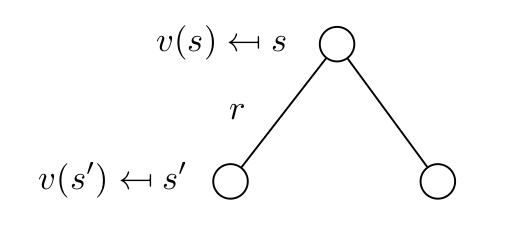
\includegraphics[width=0.5\linewidth]{figures/value.png}
    \caption{Recursive relationship between \(v(s)\) and \(v(s^{\prime} )\)}
    \label{fig:value}
\end{figure}
From the \autoref{fig:value}, we can see that the value of the state \(s\) is the
expected reward plus average of all the values of all the possible successor states.
\[
    \implies v(s) = \mathcal{R} _{s} + \gamma \sum_{s^{\prime} \in \mathcal{S} } \mathcal{P} _{ss^{\prime}} v(s^{\prime})
\]
Thus, the Bellman equation can be expreseed as a linear system of equations.
\[
    \begin{aligned}
        v &= \mathcal{R} + \gamma \mathcal{P} v  \\
        \begin{bmatrix}
             v(1) \\
             v(2) \\
             \vdots \\
             v(3) \\
        \end{bmatrix} & = 
        \begin{bmatrix}
            \mathcal{R} _{1} \\
            \mathcal{R} _{2} \\
            \vdots \\
            \mathcal{R} _{n} \\
        \end{bmatrix} + \gamma
        \begin{bmatrix}
            \mathcal{P} _{11} & \mathcal{P} _{12} & \dots & \mathcal{P} _{1n} \\
            \mathcal{P} _{21} & \mathcal{P} _{22} & \dots & \mathcal{P} _{2n} \\
            \vdots & \vdots & \ddots & \vdots \\
            \mathcal{P} _{n1} & \mathcal{P} _{n2} & \dots & \mathcal{P} _{nn} \\
        \end{bmatrix}
        \begin{bmatrix}
            v(1) \\
            v(2) \\
            \vdots \\
            v(3) \\
        \end{bmatrix} \\
        \end{aligned}
\]
SInce this is a linear system of equations, we can solve it using linear algebra.
\[
    \begin{aligned}
        v &= \mathcal{R} + \gamma \mathcal{P} v  \\
        (I - \gamma \mathcal{P} ) v &= \mathcal{R}  \\
        v &= (I - \gamma \mathcal{P} )^{-1} \mathcal{R}  \\      
    \end{aligned}
\]
Too large to compute in practice. Thus, we use iterative methods to solve
this equation.

\subsection{Markov Decision Processes}
A Markov Decision Process is a Markov Reward Process with decisions.
It is an environment in which all states are Markov. Thus the next state
that the MDp transitions to depends on the current state and the action
that the agent takes in the current state.

\begin{definition}[Markov Decision Process]
    A Markov Decision Process is a tuple \((\mathcal{S}, \mathcal{A} , \mathcal{P} , \mathcal{R} , \gamma)\)
    consisting of:
    \begin{itemize}
        \item a finite set of states \(\mathcal{S} \)
        \item a finite set of actions \(\mathcal{A} \)
        \item a state transition probability matrix \(\mathcal{P} \)
        \[
            \mathcal{P} _{ss^{\prime}}^{a} = \mathbb{P}  [S_{t+1} = s^{\prime} | S_{t} = s, A_{t} = a]  
        \]
        \item a reward function \(\mathcal{R} \)
        \[
            \mathcal{R} _{s}^{a} = \mathbb{E}  [R_{t+1} | S_{t} = s, A_{t} = a]  
        \]
        \item a discount factor \(\gamma \in [0, 1]\)
    \end{itemize}
\end{definition}
\subsubsection{Policy}
Formalises what it means to take decisions. 
\begin{definition}[Policy]
    A policy \(\pi \) is a distribution over actions given states.
    \[
        \pi (a|s) = \mathbb{P}  [A_{t} = a | S_{t} = s]  
    \]
\end{definition}
The policies fully define the behaviour of the agent. Usually,
the policies are stationary, i.e. they do not change over time.
The policies are dependent only on the current state and not on the
history of the agent.

NOTE: 
\begin{itemize}
    \item We can always recover the MRP or a Markov Process from an MDP, given
    and MDP \(\mathcal{M} = \langle \mathcal{S}, \mathcal{A} , 
    \mathcal{P} , \mathcal{R} , \gamma \rangle
    \)
    and a policy \(\pi\)
    \item If we have an policy and we sample the states using the policy,
    the state sequence is a Markov Process \( \langle \mathcal{S}, \mathcal{P} ^{\pi} \rangle \)
    
    \item Similarly, the state and reward sequence is a Markov Reward Process \( 
        \langle \mathcal{S}, \mathcal{P} ^{\pi}, \mathcal{R} ^{\pi}, \gamma \rangle \) 
\end{itemize}

where the transition dynamics and reward function are the average over the policy.
\[
    \mathcal{P}_{s,s^{\prime}}^{\pi} = \sum_{a \in \mathcal{A} } \pi (a|s) \mathcal{P}_{ss^{\prime}}^{a}  
\]
\[
    \mathcal{R}_{s}^{\pi} = \sum_{a \in \mathcal{A} } \pi (a|s) \mathcal{R}_{s}^{a}
\]

\subsubsection{Value Function and Action Value Function}
\begin{definition}[Value Function]
    The value function \(v_{\pi} (s)\) of an MDP is the expected return starting from state \(s\),
    and then following policy \(\pi \).
    \[
        v_{\pi} (s) = \mathbb{E}  [ G_{t} | S_{t} = s]  
    \]
\end{definition}
\begin{definition}[Action Value Function]
    The action-value function \(q_{\pi} (s, a)\) of an MDP is the expected return starting from state \(s\),
    taking action \(a\), and then following policy \(\pi \).
    \[
        q_{\pi} (s, a) = \mathbb{E}  [ G_{t} | S_{t} = s, A_{t} = a]  
    \] 
\end{definition}

\subsubsection{Bellman Expectation Equation for MDPs}
The action value function can be decomposed into two parts similar to the value function.
\[
        q_{\pi} (s, a) = \mathbb{E} _\pi \left[    R_{t+1} + \gamma q_\pi (S_{t+1} , A_{t+1} ) | 
        S_t = s, A_t = a \right]
\]

\begin{figure}[H]
    \centering
    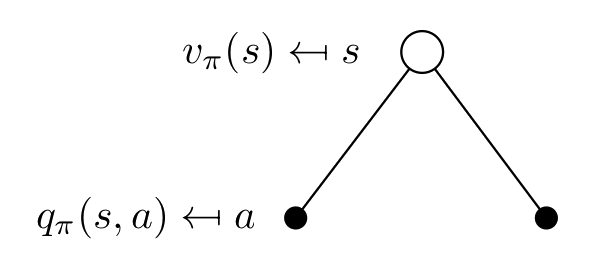
\includegraphics[width=0.5\linewidth]{figures/value-pi.png}
    \caption{The relationship between \(q_\pi\) and \(v_\pi\)}
    \label{fig:value-pi}
\end{figure}
\[
    \implies v_\pi (s) = \sum_{a \in \mathcal{A} } \pi (a|s) q_\pi (s, a)
\]
The \autoref{fig:value-pi} shows how \(q_\pi\) and \(v_\pi\) are related. The 
black dots represent the possibel actions, while the circles represent the states. The 
probabilities of chossing the action depends on the policy \(\pi \). For each of 
the action we might take from state \(s\), we have a \(q\)-value \(q_\pi (s, a)\), that describes
the expected return from taking action \(a\) in state \(s\). Thus, the value of the state \(s\), is calculated by taking the average of all the q values
after doing a one step look-ahead.
Simlarly the \(q\) value of the state action pair is calculated by averaging the value of the
state that we might transition into according to the MDP dynamics, after taking action \(a\) 
from state \(s\). The tree backup diagram for the \(q\) value is shown in \autoref{fig:q-value}.
\begin{figure}[H]
    \centering
    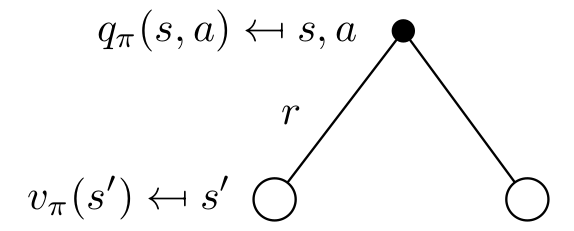
\includegraphics[width=0.5\linewidth]{figures/action-pi.png}
    \caption{The relationship between \(q_\pi\) and \(v_\pi\)}
    \label{fig:q-value}
\end{figure}
\[
    \implies q_\pi (s, a) = \mathcal{R} _{s}^{a} + \gamma \sum_{s^{\prime} \in \mathcal{S} } \mathcal{P} _{ss^{\prime}}^{a} v_\pi (s^{\prime} )
\]

Combining \autoref{fig:value-pi} and \autoref{fig:q-value}, 
we get \autoref{fig:value-value} a recursive relationship between \(v(s)\) and \(v(s^{\prime} )\).
Thus, we are averaging over the policy, and the transition dynamics of the MDP.
\[
    v_\pi (s) = \sum_{a \in \mathcal{A} } \pi (a|s) \left( 
        \mathcal{R} _{s}^{a} + \gamma \sum_{s^{\prime} \in \mathcal{S} 
        } \mathcal{P} _{ss^{\prime}}^{a} v_\pi (s^{\prime} ) \right)  
\]
\begin{figure}
    \centering
    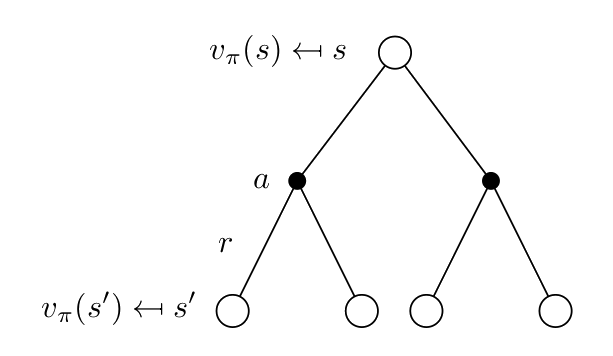
\includegraphics[width=0.5\linewidth]{figures/value-value.png}
    \caption{Recursive relationship between \(v(s)\) and \(v(s^{\prime} )\)}
    \label{fig:value-value}
\end{figure}

The Bellman Expectation Equation can be written concisely in matrix form.
\[
    \begin{aligned}
        v_{\pi} &= \mathcal{R} ^{\pi} + \gamma \mathcal{P} ^{\pi} v_{\pi}  \\
        v_{\pi} &= \left( 
            I - \gamma \mathcal{P} ^{\pi}
         \right) ^{-1} \mathcal{R} ^{\pi}  \\
    \end{aligned}
\]

\subsubsection{Optimal Value Function}
\begin{definition}[Optimal Value Function]
    The optimal value function \(v_{*} (s)\) is the maximum value function over all policies.
    \[
        v_{*} (s) = \max_{\pi} v_{\pi} (s)  
    \]
    The optimal action value function \(q_{*} (s, a)\) is the maximum
    action value function over all policies.
    \[
        q_{*} (s, a) = \max_{\pi} q_{\pi} (s, a)
    \]
\end{definition}
If we know the optimal action-value function, we can easily construct the optimal policy. 
So, we can say that the RL problem is solved if we know \(q_{*} (s, a)\). The way to compare
policies is to compare the value functions of the policies.
\[
    \pi \geq \pi^{\prime} \iff v_{\pi} (s) \geq v_{\pi^{\prime}} (s) \quad \forall s \in \mathcal{S}  
\]
\begin{theorem}[Optimal Policy]
    For any MDP:
    \begin{itemize}
        \item There exists an optimal policy \(\pi_{*} \) that is better than or equal to all other policies,
        \[
            \pi_{*} \geq \pi \quad \forall \pi  
        \]
        \item All optimal policies achieve the optimal value function,
        \[
            v_{\pi_{*}} (s) = v_{*} (s) \quad \forall s \in \mathcal{S}  
        \]
        \item All optimal policies achieve the optimal action-value function,
        \[
            q_{\pi_{*}} (s, a) = q_{*} (s, a) \quad \forall s \in \mathcal{S} , \forall a \in \mathcal{A}  
        \]
    \end{itemize}
\end{theorem}
The optimal policy can be found by maximising over \(q_{*} (s, a)\).
\[
    \pi_{*} (a|s) = 
    \begin{cases}
        1 & \text{if } a = \argmax\limits_{a \in \mathcal{A} } q_{*} (s, a) \\
        0 & \text{otherwise} \\
    \end{cases}
\]
\subsubsection{Bellman Optimality Equation}
The optimal vale functions are recursively related by the Bellman
optimality equation.
Before we looked at the Expectation equation, looking at the average
value of the state. Now, we look at the maximum value of the state. 
Thus, taking an action \(a\) from the state \(s\), we choose the action
that has the maximum state-action value. The tree backup diagram for the
optimal value function is shown in \autoref{fig:v-star}
\[
    v_{*} (s) = \max_{a \in \mathcal{A} } q_{*} (s, a)  
\] 
\begin{figure}[H]
    \centering
    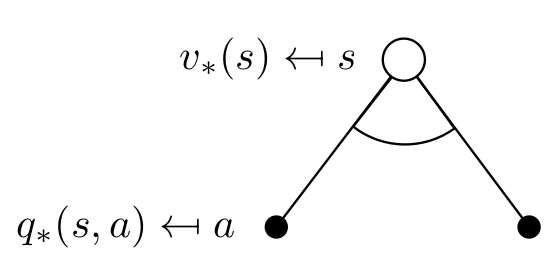
\includegraphics[width=0.5\linewidth]{figures/v-star.png}
    \caption{Bellman Optimality Equation for \(v_{*} (s)\)}
    \label{fig:v-star}
\end{figure}

Similarly, the same argument can be made for the optimal action value function,
with its tree backup diagram shown in \autoref{fig:q-star}.
\[
    q_{*} (s, a) = \mathcal{R} _{s}^{a} + \gamma \sum_{s^{\prime} \in \mathcal{S} } \mathcal{P} _{ss^{\prime}}^{a} v_{*} (s^{\prime} )
\]
\begin{figure}[H]
    \centering
    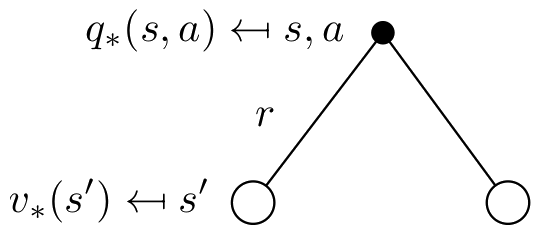
\includegraphics[width=0.5\linewidth]{figures/q-star.png}
    \caption{Bellman Optimality Equation for \(q_{*} (s, a)\)}
    \label{fig:q-star}
\end{figure}

Combining \autoref{fig:v-star}
 and \autoref{fig:q-star}
 , we get \autoref{fig:qv-star},
with the Bellman Optimality Equation for \(v_{*} (s)\), being written
in a recursive form as
\[
    v_{*} (s) = \max_{a \in \mathcal{A} } \left( 
        \mathcal{R} _{s}^{a} + \gamma \sum_{s^{\prime} \in \mathcal{S} } \mathcal{P} _{ss^{\prime}}^{a} v_{*} (s^{\prime} )
     \right)  
\]
\begin{figure}[H]
    \centering
    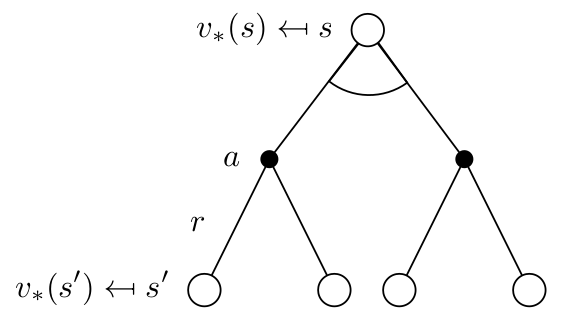
\includegraphics[width=0.5\linewidth]{figures/qv-star.png}
    \caption{Recursive relationship between \(v_{*} (s)\) and \(v_{*} (s^{\prime} )\)} 
    \label{fig:qv-star}
\end{figure}
Similarly, the Bellman Optimality Equation for \(q_{*} (s, a)\) can be written in
a recursive form as
\[
    q_{*} (s, a) = \mathcal{R} _{s}^{a} + \gamma \sum_{s^{\prime}
     \in \mathcal{S} } \mathcal{P} _{ss^{\prime}}^{a} 
     \max_{a^{\prime} \in \mathcal{A} } q_{*} (s^{\prime} , a^{\prime} )
\]

\subsubsection*{Solving the Bellman Optimality Equation}
\begin{itemize}
    \item Bellman optimality equation is a non-linear equation
    \item It can be solved using iterative methods
    \begin{itemize}
        \item Value Iteration
        \item Policy Iteration
        \item Q-learning
        \item Sarsa
    \end{itemize}
\end{itemize}